\documentclass{beamer}

\usepackage[sfdefault]{cabin}
\usepackage[utf8]{inputenc}
\usepackage[T1]{fontenc}
\usepackage[french]{babel}
\usepackage{xcolor}
\usepackage{caption}
\usepackage{graphicx}
%Police
%\usepackage[sfdefault]{roboto}
\usepackage[sfdefault]{FiraSans}

\definecolor{modernblue}{RGB}{70,130,180} 
\definecolor{modernvert}{RGB}{0, 80, 0} 

\usetheme{Madrid}

\usecolortheme[named=modernblue]{structure}

\setbeamertemplate{caption}{\insertcaption} % Utiliser le format de légende par défaut de Beamer

\title{Application des séries chronologiques sur les données Dataset\_CB.csv}
\author{Ivanhoé \& Youness}
\date{11 janvier 2024}

\renewcommand{\thesection}{\Roman{section}}\renewcommand{\thesubsection}{\arabic{subsection} }\renewcommand{\thesubsubsection}{\alph{subsubsection} }

\newcommand{\C}{\mathbb{C}}\newcommand{\R}{\mathbb{R}}\newcommand{\Q}{\mathbb{Q}}\newcommand{\Z}{\mathbb{Z}}\newcommand{\N}{\mathbb{N}}\newcommand{\V}{\overrightarrow}\newcommand{\Cs}{\mathscr{C}}\newcommand{\Ps}{\mathscr{P}}\newcommand{\Rs}{\mathscr{R}}\newcommand{\Gs}{\mathscr{G}}\newcommand{\Ds}{\mathscr{D}}\newcommand{\happy}{\huge\smiley}\newcommand{\sad}{\huge\frownie}\newcommand{\alors}{\Large\Rightarrow}\newcommand{\equi}{\Leftrightarrow}
\newcommand{\disp}{\displaystyle}\newcommand{\Pro}{\mathbb{P}}


\newtheorem{thm}{Théorème}
\newtheorem{rmq}{Remarque}
\newtheorem{prop}{Propriété}
\newtheorem{cor}{Corollaire}
\newtheorem{lem}{Lemme}
\newtheorem{prop-def}{Propriété-définition}
\newtheorem{con}{Conclusion}

\theoremstyle{definition}

\newtheorem{defi}{Définition}
\newtheorem{intro}{Initialisation}
\newtheorem{boucle}{Boucle principale}
\newtheorem{ex}{Exemple}
\newtheorem*{rap}{Rappel}
\newtheorem{cex}{Contre-exemple}
\newtheorem{exer}{Exercice} % \large {\fontfamily{ptm}\selectfont EXERCICE}
\newtheorem{nota}{Notation}
\newtheorem{ax}{Axiome}
\newtheorem{appl}{Application}
\newtheorem{csq}{Conséquence}
\def\di{\displaystyle}



\begin{document}
\begin{frame}[plain]
    \maketitle
\end{frame}


\begin{frame}
\frametitle{Introduction}
\hfill\\[-0.75cm]
\begin{figure}
	\centering
	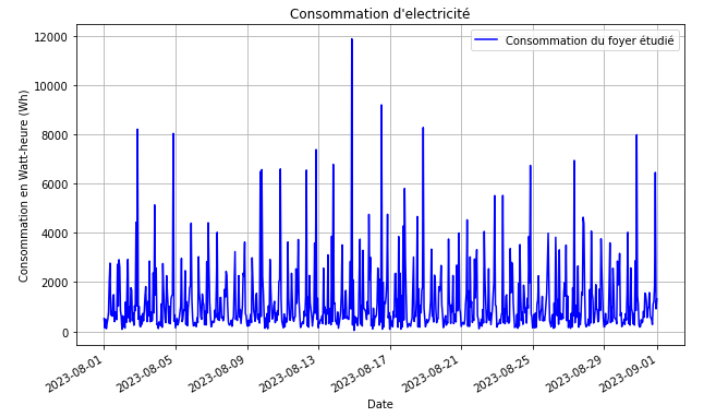
\includegraphics[scale=0.35]{1.png}\\[-0.25cm]
	\caption*{Voici une série chronologique de données pseudo-réelles issue d'une consommation EDF d'un foyer.}
\end{figure}

\textcolor{modernvert}{\textbf{Problématique :}} Comment prédire à l'horizon de 7 jours la
consommation électrique du foyer sur la première semaine de septembre 2023 ?
\end{frame}

\begin{frame}
	\tableofcontents
\end{frame}

\section{Partie preprocessing}
\begin{frame}
	\frametitle{Renommer les colonnes et passer au format date}
		\begin{minipage}[c]{1\linewidth}
		\begin{minipage}[c]{0.4\linewidth}\centering\begin{figure}
				\centering
				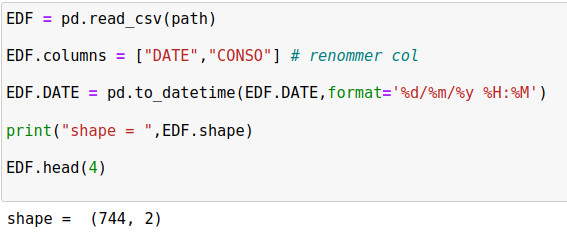
\includegraphics[scale=0.28]{2.png}
				\caption*{Chargement des données}
				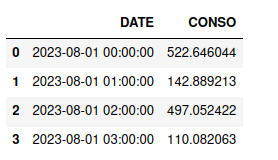
\includegraphics[width=1\linewidth]{3.png}
				\caption*{Dataset EDF}
		\end{figure}\end{minipage}\hfill 
		\begin{minipage}[c]{0.5\linewidth}\centering\begin{figure}
				\begin{center}
					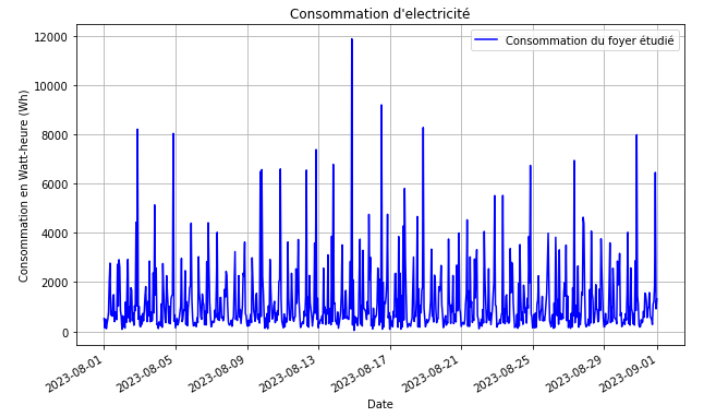
\includegraphics[width=1\linewidth]{1.png}			
					\caption*{Consommation du foyer}
				\end{center}
				
		\end{figure}\end{minipage}
	\end{minipage}	
\end{frame}

\begin{frame}
	\frametitle{Passage au log pour réduire la variabilité de la série}
	\begin{minipage}[c]{1\linewidth}
		\begin{minipage}[c]{0.4\linewidth}\centering\begin{figure}
				\centering
				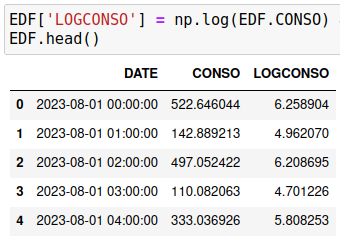
\includegraphics[width=1\linewidth]{4.png}
				\caption*{Dataset EDF}
		\end{figure}\end{minipage}\hfill 
		\begin{minipage}[c]{0.58\linewidth}\centering\begin{figure}
				\begin{center}
					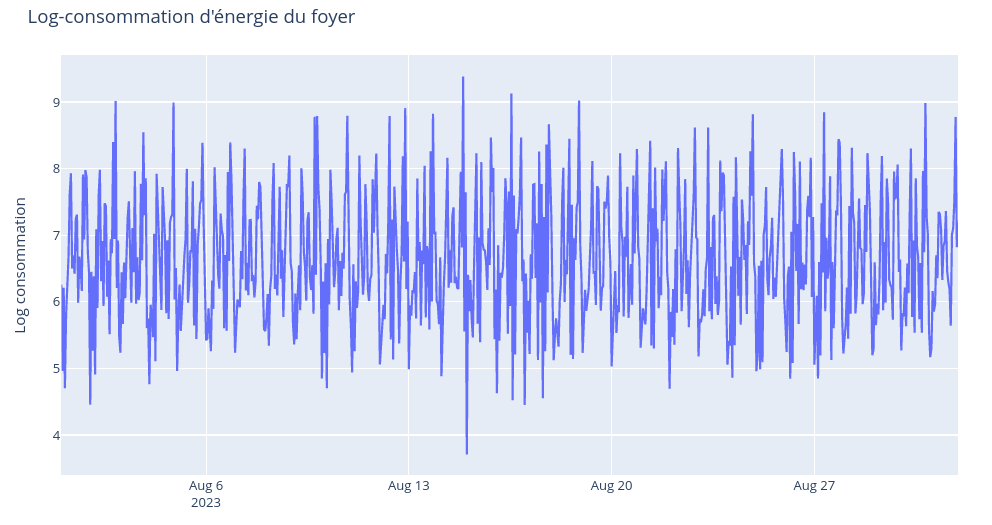
\includegraphics[width=1\linewidth]{5.png}			
					\caption*{Log-consommation du foyer}
				\end{center}
				
		\end{figure}\end{minipage}
	\end{minipage}
	
\end{frame}
\section{Stationnarité et vérification}
\begin{frame}
	\frametitle{Étude de la stationnarité de la log-consommation}
	\begin{minipage}[t]{1\linewidth}
	\begin{minipage}[c]{0.58\linewidth}\centering\begin{figure}
			\centering
			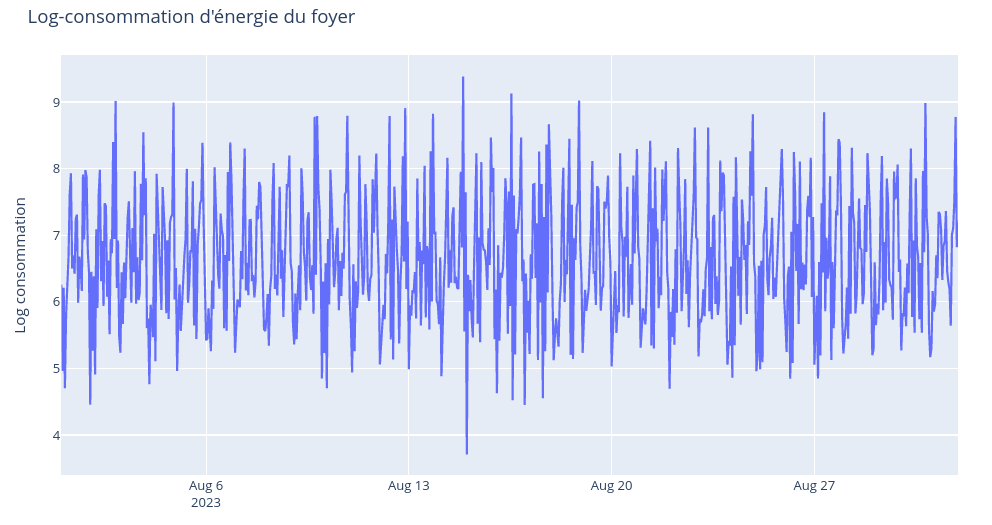
\includegraphics[width=1\linewidth]{5.png}
			\caption*{Log-consommation du foyer}
	\end{figure}\end{minipage}\hfill 
	\begin{minipage}[c]{0.4\linewidth}\centering\begin{figure}
			\begin{center}
				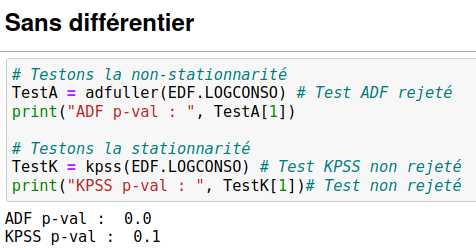
\includegraphics[width=1\linewidth]{6.png}			
				\caption*{Tests ADF et KPSS}
			\end{center}
			
	\end{figure}\end{minipage}
\end{minipage}
	
\end{frame}

\begin{frame}
	\frametitle{Étude de la stationnarité de la log-consommation avec une différentiation saisonnière}
	\begin{minipage}[t]{1\linewidth}
		\begin{minipage}[c]{0.55\linewidth}\centering\begin{figure}
				\centering
				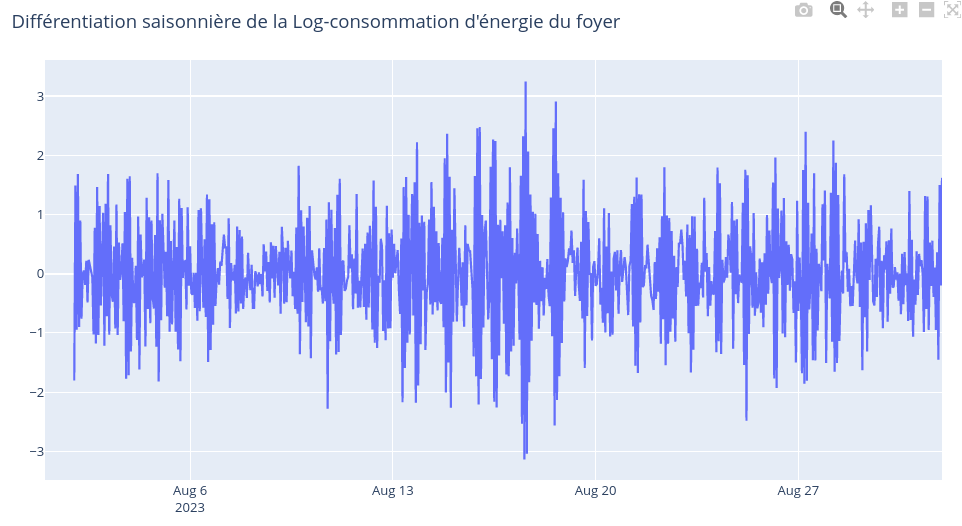
\includegraphics[width=1\linewidth]{8.png}
				\caption*{Différentielle saisonnière log-consommation du foyer}
		\end{figure}\end{minipage}\hfill 
		\begin{minipage}[c]{0.44\linewidth}\centering\begin{figure}
				\begin{center}
					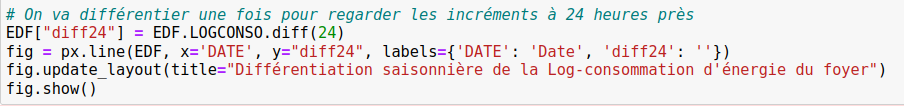
\includegraphics[width=1\linewidth]{7.png}
					\caption*{Différentiation D=24}
					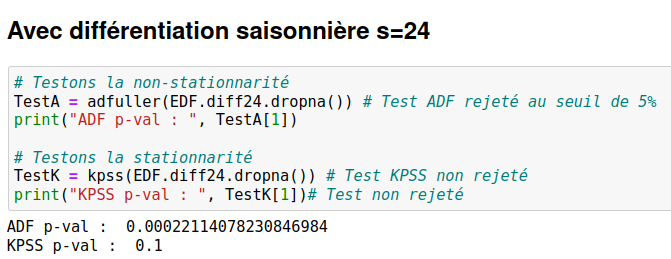
\includegraphics[width=1\linewidth]{9.png}			
					\caption*{Tests ADF et KPSS}
				\end{center}
				
		\end{figure}\end{minipage}
		\begin{rmq}
		Attention avec les tests de stationnarité, l'hétéroscédasticité n'est pas toujours repérée.
	\end{rmq}
	\end{minipage}
	
\end{frame}

\section{Étude des corrélations}

\begin{frame}
	\frametitle{Étude des corrélations sur la série passée au log }
	\begin{minipage}[t]{1\linewidth}
		\centering
		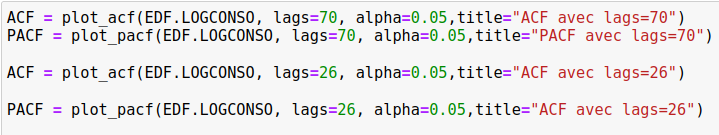
\includegraphics[width=0.8\linewidth]{10.png}
		\begin{minipage}[c]{0.48\linewidth}\centering\begin{figure}
				\centering
				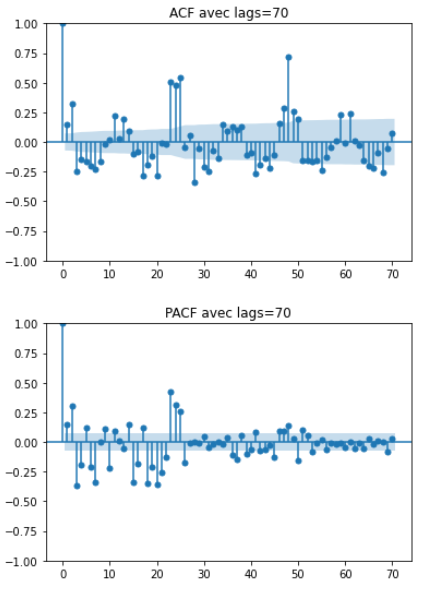
\includegraphics[width=0.75\linewidth]{11.png}	
		\end{figure}\end{minipage}\hfill 
		\begin{minipage}[c]{0.48\linewidth}\centering\begin{figure}
				\begin{center}
					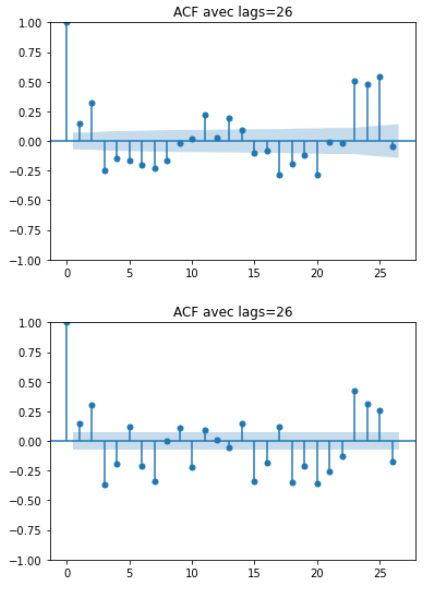
\includegraphics[width=0.75\linewidth]{12.png}			
				\end{center}
				
		\end{figure}\end{minipage}
	\end{minipage}

\end{frame}

\section{Recherche de modèles significatifs}

\begin{frame}
	\frametitle{Recherche de modèles à l'aide de la fonction AUTO\_ARIMA sous certaines contraintes}
	\begin{minipage}[t]{1\linewidth}
		\centering

		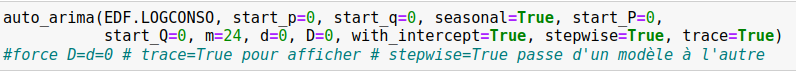
\includegraphics[width=1\linewidth]{13.png}\\
		
		Best model:  ARIMA(5,0,0)(1,0,2)[24] intercept\\[0.5cm]
		
		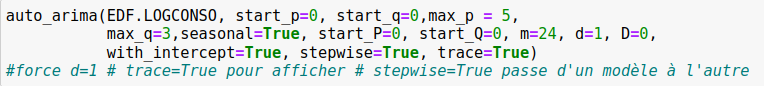
\includegraphics[width=1\linewidth]{14.png}\\
		Best model:  ARIMA(1,1,0)(1,0,0)[24]\\[1cm]          
	\end{minipage}
	\begin{rmq}
		Commandes qui mettent beaucoup de temps à s'exécuter.
	\end{rmq}
\end{frame}


\begin{frame}
	\frametitle{Modèle 1 : SARIMAX(EDF.LOGCONSO, order=(5, 0, 0), seasonal\_order=(1, 0, 2, 24), trend=None)}
	\begin{minipage}[t]{1\linewidth}
		\centering
		\begin{minipage}[c]{0.55\linewidth}\centering\begin{figure}
				\centering
				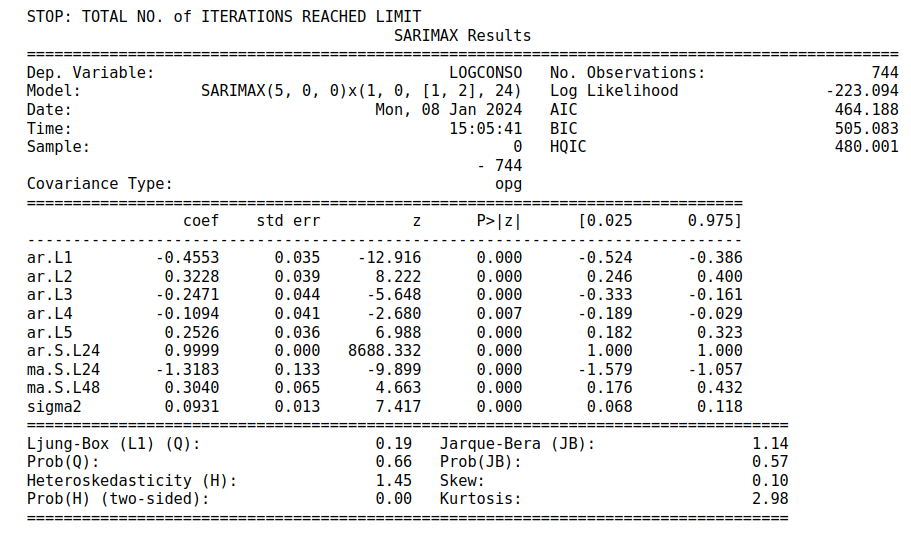
\includegraphics[width=1\linewidth]{16.png}	
		\end{figure}\end{minipage}\hfill 
		\begin{minipage}[c]{0.44\linewidth}\centering\begin{figure}
				\begin{center}
					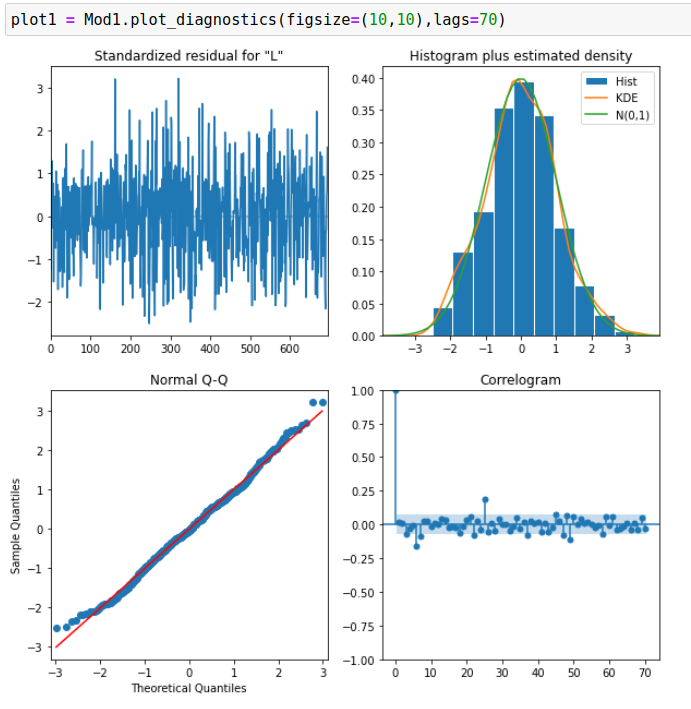
\includegraphics[width=1\linewidth]{17.png}			
				\end{center}
				
		\end{figure}\end{minipage}
	\end{minipage}	
\end{frame}

\begin{frame}
	\frametitle{Modèle 2 : SARIMAX(EDF.LOGCONSO, order=(5, 0, 0), seasonal\_order=(2, 0, 2, 24), trend=None)}
	\begin{minipage}[t]{1\linewidth}
		\centering
		\begin{minipage}[c]{0.55\linewidth}\centering\begin{figure}
				\centering
				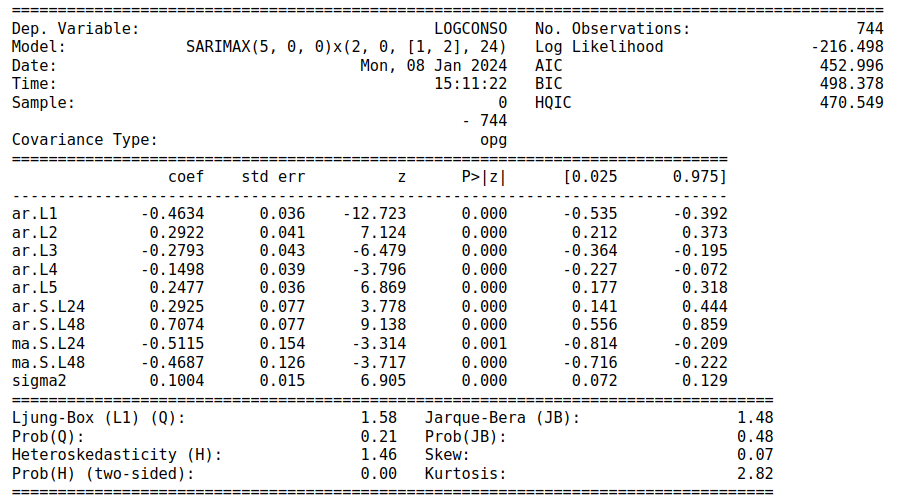
\includegraphics[width=1\linewidth]{18.png}	
		\end{figure}\end{minipage}\hfill 
		\begin{minipage}[c]{0.44\linewidth}\centering\begin{figure}
				\begin{center}
					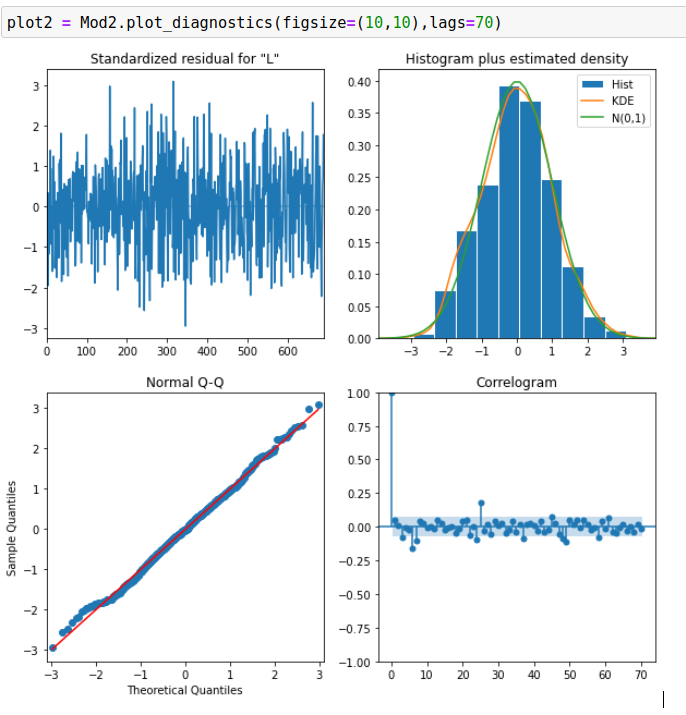
\includegraphics[width=1\linewidth]{19.png}			
				\end{center}
				
		\end{figure}\end{minipage}
	\end{minipage}	
\end{frame}

\begin{frame}
	\frametitle{Modèle 3 : SARIMAX(EDF.LOGCONSO, order=(7, 0, 0), seasonal\_order=(2, 0, 2, 24), trend=None)}
	\begin{minipage}[t]{1\linewidth}
		\centering
		\begin{minipage}[c]{0.55\linewidth}\centering\begin{figure}
				\centering
				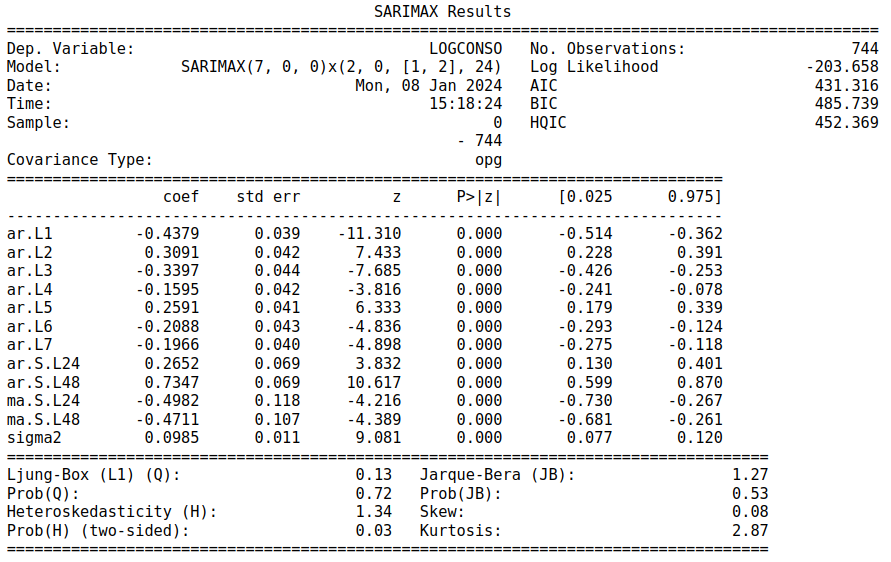
\includegraphics[width=1\linewidth]{20.png}	
		\end{figure}\end{minipage}\hfill 
		\begin{minipage}[c]{0.44\linewidth}\centering\begin{figure}
				\begin{center}
					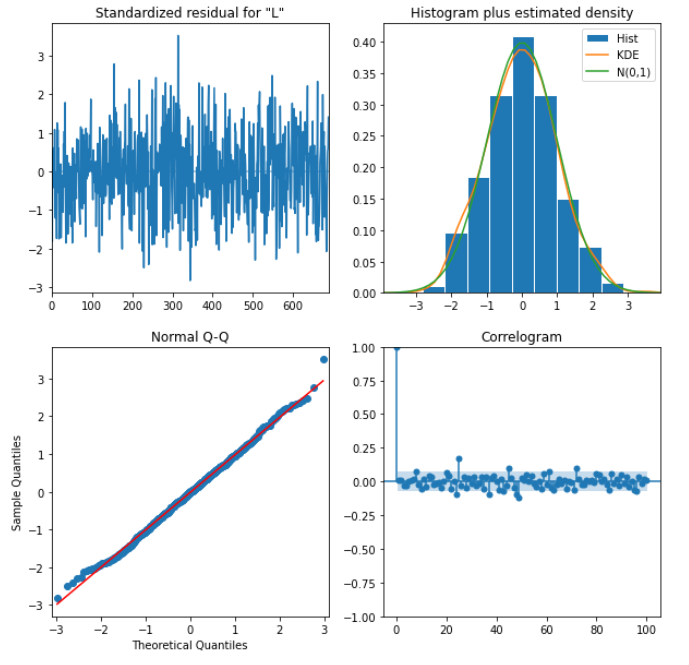
\includegraphics[width=1\linewidth]{21.png}			
				\end{center}
				
		\end{figure}\end{minipage}
	\end{minipage}	
\end{frame}

\begin{frame}
	\frametitle{Modèle 4 : SARIMAX(EDF.LOGCONSO, order=(8, 1, 0), seasonal\_order=(2, 0, 1, 24), trend=None)}
	\begin{minipage}[t]{1\linewidth}
		\centering
		\begin{minipage}[c]{0.55\linewidth}\centering\begin{figure}
				\centering
				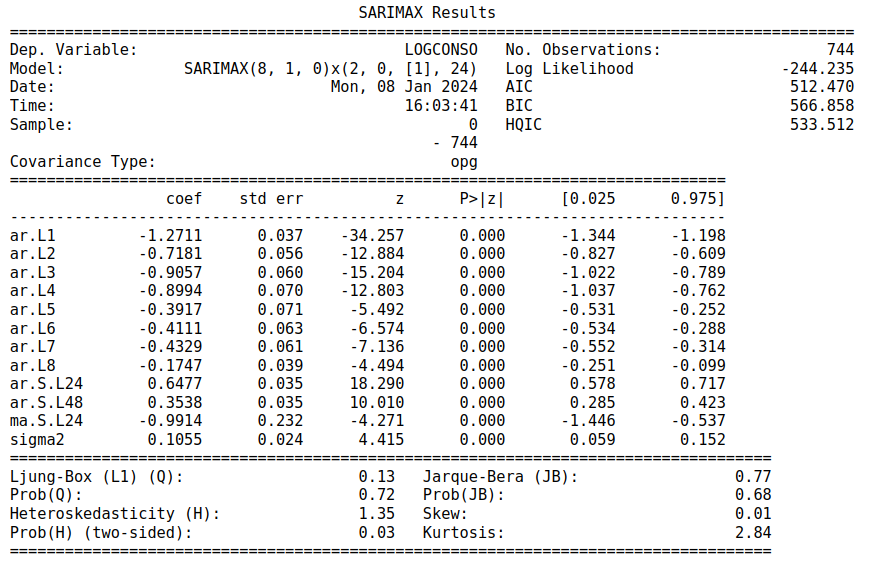
\includegraphics[width=1\linewidth]{22.png}	
		\end{figure}\end{minipage}\hfill 
		\begin{minipage}[c]{0.44\linewidth}\centering\begin{figure}
				\begin{center}
					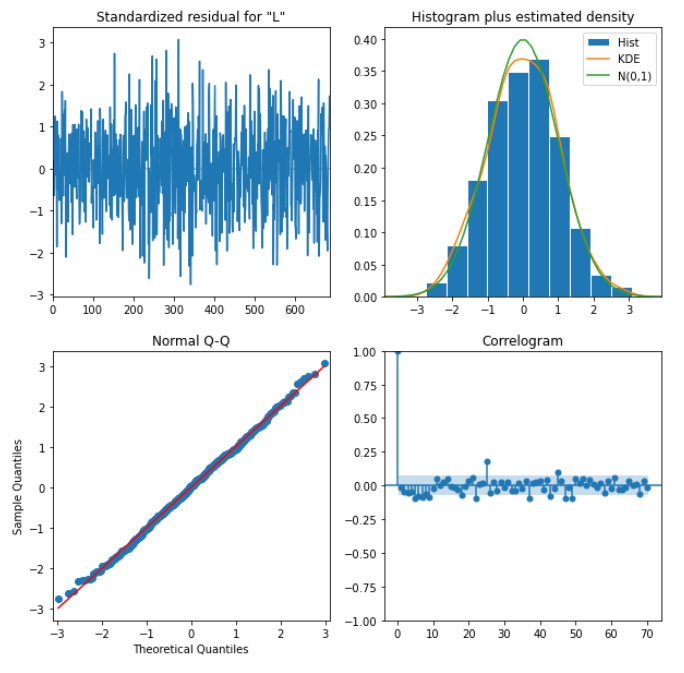
\includegraphics[width=1\linewidth]{23.png}			
				\end{center}
				
		\end{figure}\end{minipage}
	\end{minipage}	
\end{frame}

\begin{frame}
	\begin{figure}
		\centering
		\begin{minipage}{\linewidth}
			\centering
			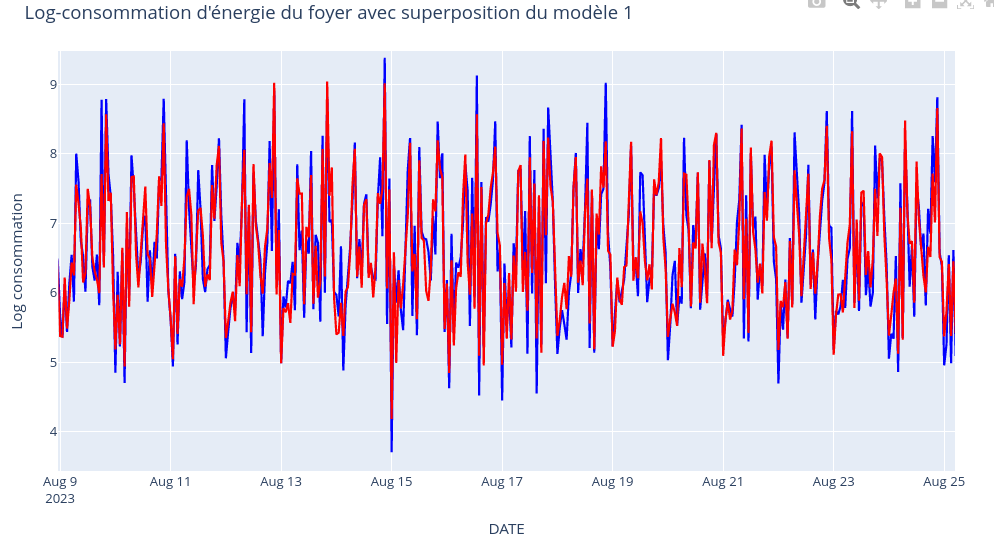
\includegraphics[width=0.65\linewidth]{24.png}
			%\caption*{Modèle 1}
		\end{minipage}
		\\
		\begin{minipage}{\linewidth}
			\centering
			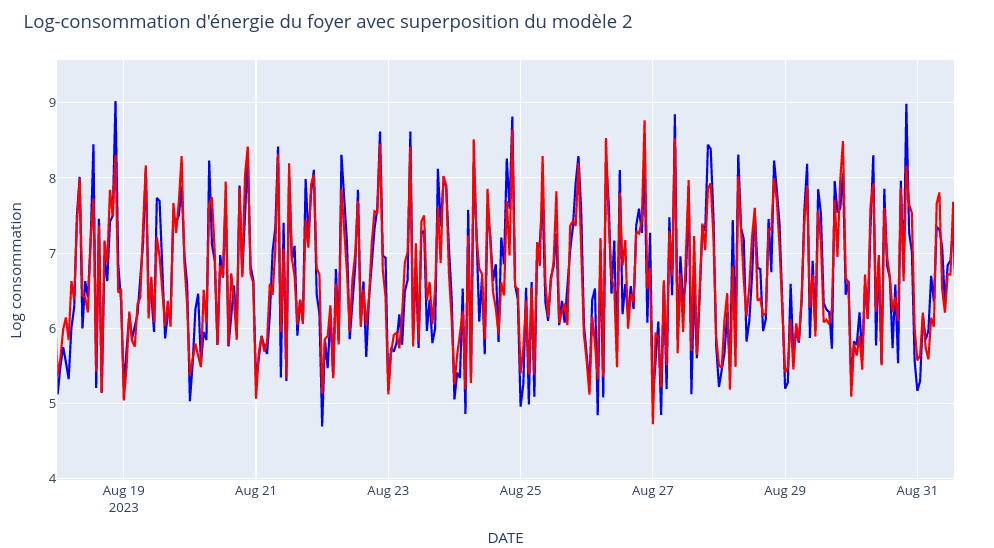
\includegraphics[width=0.65\linewidth]{25.png}
			%\caption*{Modèle 2}
		\end{minipage}
	\end{figure}
\end{frame}

\begin{frame}
	\begin{figure}
		\centering
		\begin{minipage}{\linewidth}
			\centering
			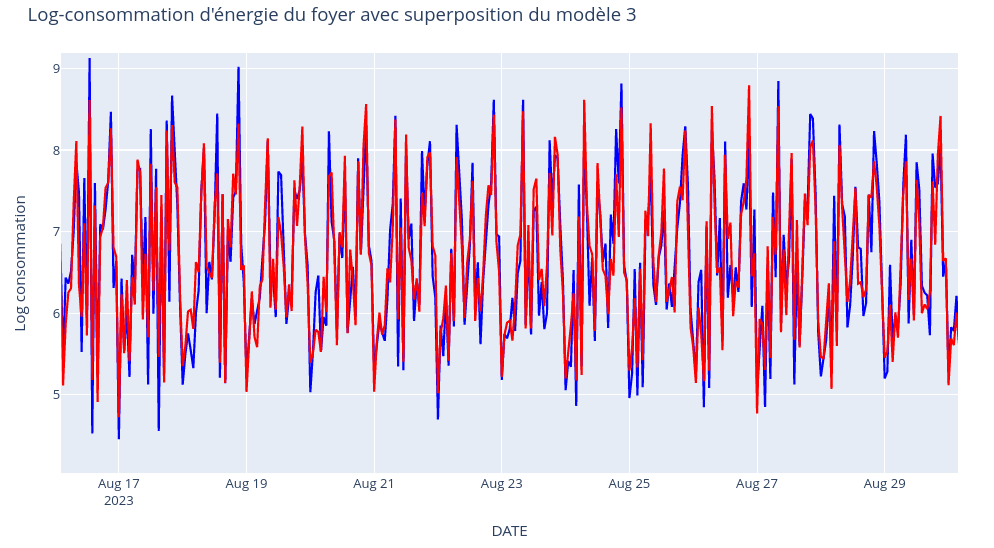
\includegraphics[width=0.65\linewidth]{26.png}
			%\caption*{Modèle 1}
		\end{minipage}
		\\
		\begin{minipage}{\linewidth}
			\centering
			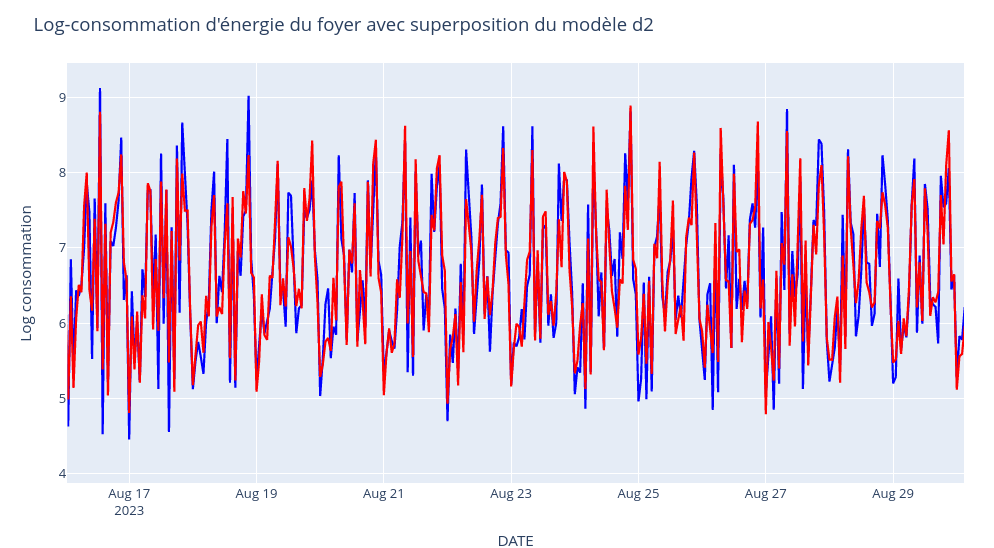
\includegraphics[width=0.65\linewidth]{27.png}
			%\caption*{Modèle 2}
		\end{minipage}
	\end{figure}
\end{frame}

\section{Cross validation et évaluation}

\begin{frame}
	\frametitle{Cross validation : une partie train et une partie test, entraînement sur les données train}
	\begin{minipage}[t]{1\linewidth}
		\centering\hfill\\[-0.5cm]
		\begin{figure}	
		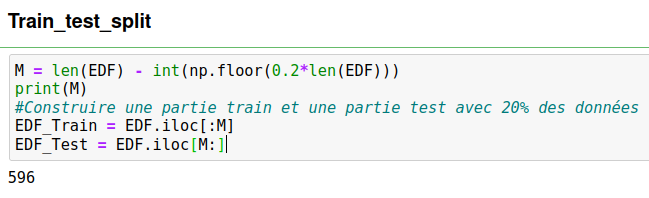
\includegraphics[width=0.6\linewidth]{28.png}	
		\caption*{Test dataset correspondant à 20\% des données}
		
		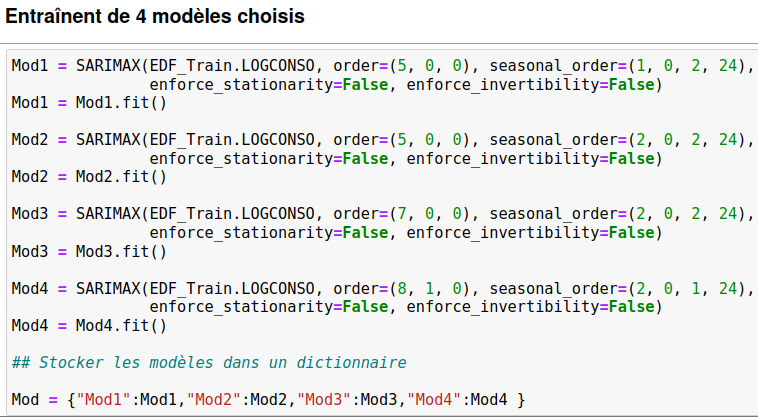
\includegraphics[width=0.6\linewidth]{29.png}		
				
				
		\end{figure}
	\end{minipage}	
\end{frame}

\begin{frame}
	\frametitle{Prédiction sur la partie test et évaluation avec certaines métriques}
	\begin{minipage}[t]{1\linewidth}
		\centering\hfill\\[-0.5cm]
		\begin{figure}	
			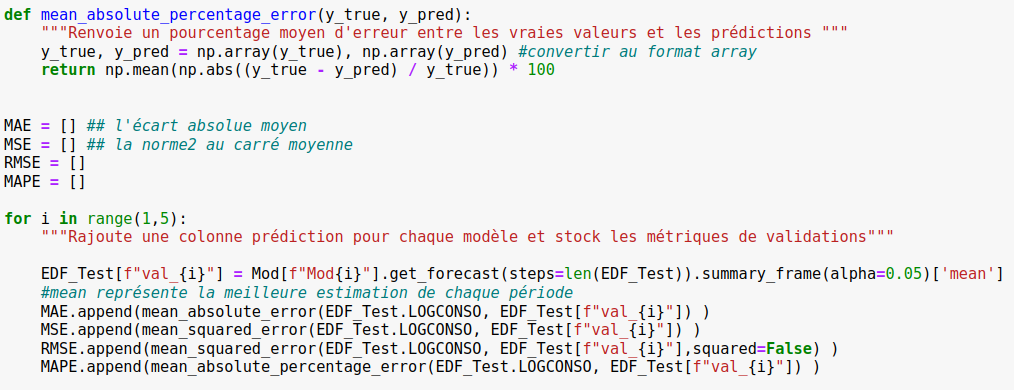
\includegraphics[width=1\linewidth]{30.png}	
			\caption*{}
			
		\end{figure}
	\end{minipage}	
\end{frame}

\begin{frame}
	\frametitle{Dataset test complété avec les prédictions sur la partie test "Forcast\_test" }
	\begin{minipage}[t]{1\linewidth}
		\centering\hfill\\[-1cm]
		\begin{figure}	
			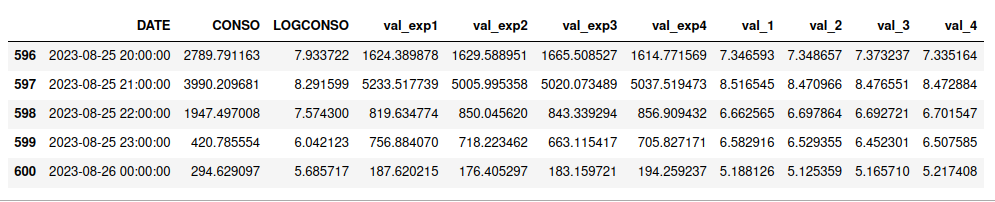
\includegraphics[scale =0.35]{34.png}	
		\end{figure}\hfill\\
	\begin{rmq}
		
		Le meilleur modèle sera celui qui minimise les métriques telles que la MAE et la MSE dans notre cas. En réalité, une métrique différente pourrait être choisie selon la demande d'un métier spécialiste sur la consommation d'électricité.
	\end{rmq}
	\end{minipage}	
\end{frame}

\begin{frame}
	\frametitle{Comparaison des métriques pour l'évaluation des différents modèles}
	\begin{minipage}[t]{1\linewidth}
		\centering
		\begin{minipage}[c]{0.49\linewidth}\centering\begin{figure}
				\centering
				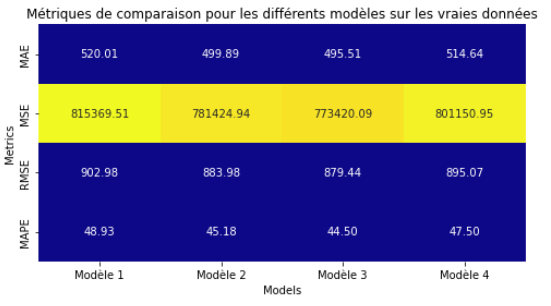
\includegraphics[width=1\linewidth]{32.png}	
		\end{figure}\end{minipage}\hfill 
		\begin{minipage}[c]{0.49\linewidth}\centering\begin{figure}
				\begin{center}
					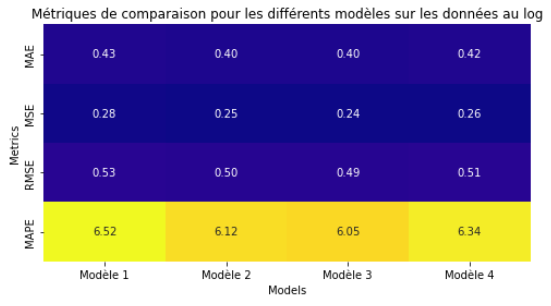
\includegraphics[width=1\linewidth]{33.png}			
				\end{center}
				
		\end{figure}\end{minipage}
	\end{minipage}	
\end{frame}

\section{Prédiction avec le meilleur modèle}

\begin{frame}
	\frametitle{Prédiction sur la partie test et évaluation avec certaines métriques}
	\begin{minipage}[t]{1\linewidth}
		\centering\hfill\\[-0.5cm]
		\begin{figure}	
			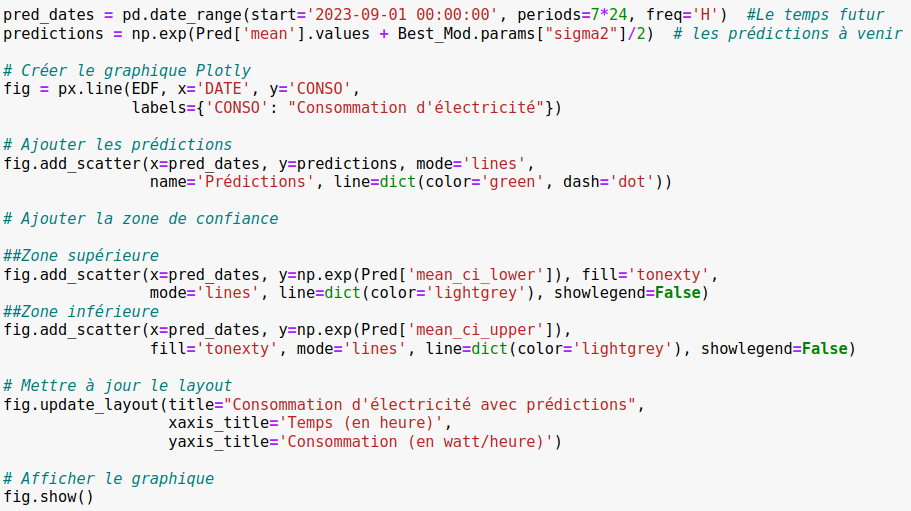
\includegraphics[width=1\linewidth]{35.png}	
			\caption*{}
			
		\end{figure}
	\end{minipage}	
\end{frame}

\begin{frame}
	\frametitle{Représentation graphique des prédictions avec les intervalles de confiance à 95\%}
	\begin{minipage}[t]{1.03\linewidth}
		\centering\hfill\\[-0.5cm]
		\begin{figure}	
			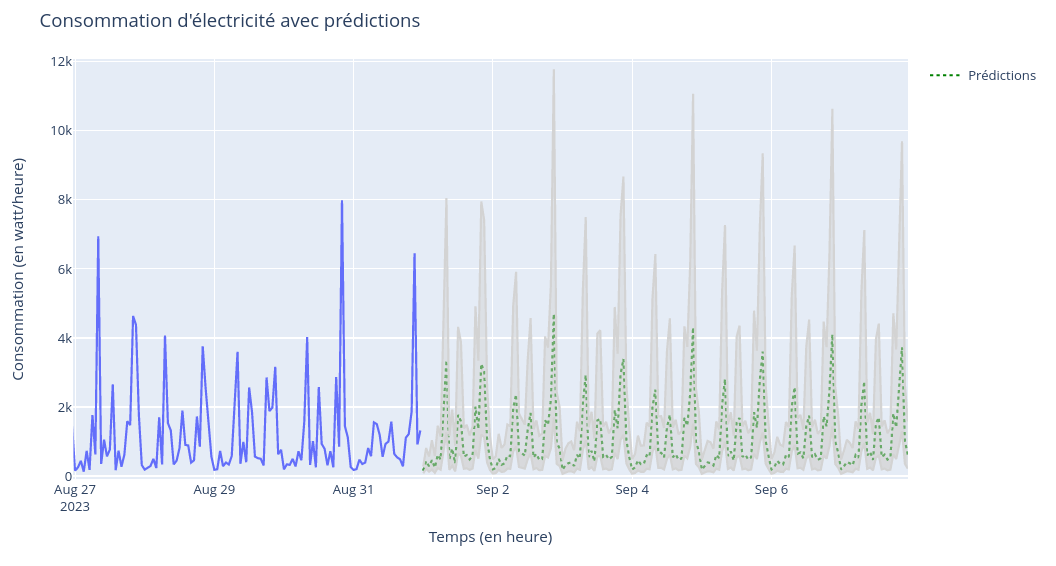
\includegraphics[width=1\linewidth]{36.png}	
			\caption*{}
			
		\end{figure}
	\end{minipage}	
\end{frame}

\section{Conclusion}

\begin{frame}
\begin{con}
	\begin{enumerate}
		\item La RMSE est relativement importante et l'indicateur MAPE sur les données réelle n'est pas non plus très bon (40\% d'erreur en moyenne).
		\item Le traitement des températures, la nébulosité ainsi que la pression atmosphérique pourraient être intégrés dans notre modèle.
		\item Trouver le caractère saisonnier avec une méthode plus précise comme la transformée de Fourier.
		\item Tester d'autres méthodes pour traiter les données (ex : réseau de neurones RNN)
	\end{enumerate}
\end{con}
		
\end{frame}


\end{document}








